\documentclass[tikz,border=10pt]{standalone}
\usepackage{enumitem} % For compact itemize lists
\usetikzlibrary{arrows.meta, positioning}

\definecolor{uzkblau}    {RGB} {0,81,118}

\begin{document}

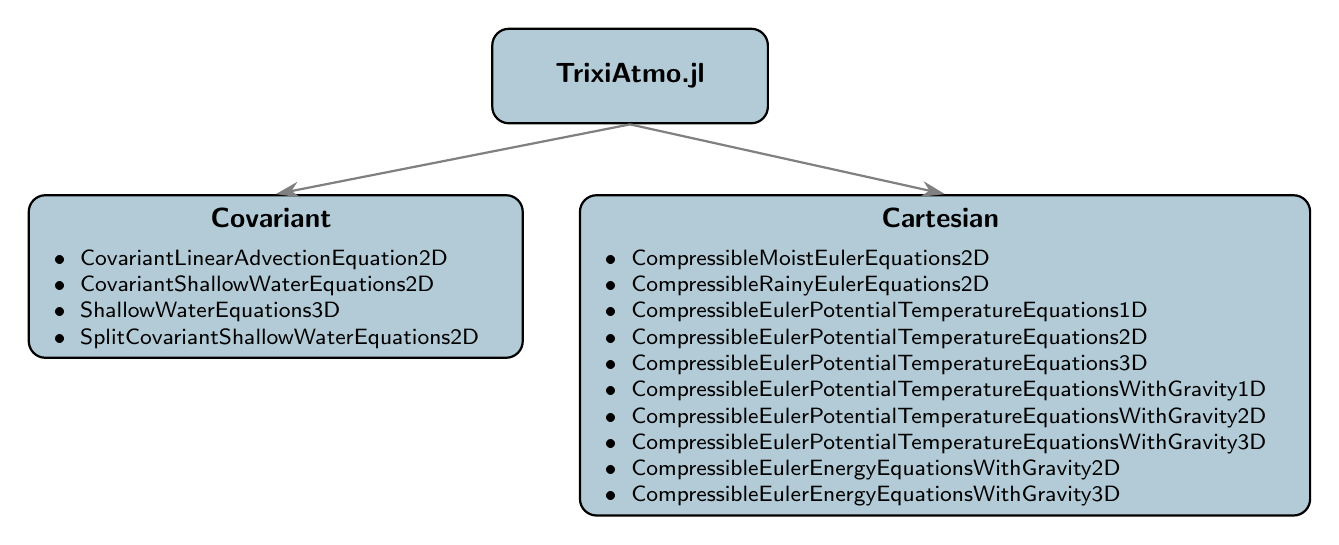
\begin{tikzpicture}[
    % Define the style for the tiles
    tile/.style={
        rectangle,
        rounded corners=6pt,
        draw=black,
        thick,
        fill=uzkblau!30,
        align=center,
        minimum height=1.2cm,
        font=\sffamily
    },
    % Define the style for the arrows
    arrow/.style={
        ->,
        thick,
        color=gray,
        >={Stealth[length=3mm, width=2mm]}
    }
]

    % ---------------------------------------------------
    % 1. MAIN CENTER NODE
    % ---------------------------------------------------
    \node[tile, minimum width=3.5cm] (trixi) at (0, 0) {\textbf{TrixiAtmo.jl}};

    % ---------------------------------------------------
    % 2. SOUTH-WEST AND SOUTH-EAST NODES
    % ---------------------------------------------------
    % Cartesian Node (South-West)
    \node[tile,anchor=north] (cartesian) at (4.0, -1.5) {
        \begin{tabular}{c}
            \textbf{Cartesian} \\[1ex]
            \begin{minipage}{8.5cm}
                \footnotesize
                \begin{itemize}[leftmargin=*, nosep]
                    \item CompressibleMoistEulerEquations2D
                    \item CompressibleRainyEulerEquations2D
                    \item CompressibleEulerPotentialTemperatureEquations1D
                    \item CompressibleEulerPotentialTemperatureEquations2D
                    \item CompressibleEulerPotentialTemperatureEquations3D
                    \item CompressibleEulerPotentialTemperatureEquationsWithGravity1D
                    \item CompressibleEulerPotentialTemperatureEquationsWithGravity2D
                    \item CompressibleEulerPotentialTemperatureEquationsWithGravity3D
                    \item CompressibleEulerEnergyEquationsWithGravity2D
                    \item CompressibleEulerEnergyEquationsWithGravity3D
                \end{itemize}
            \end{minipage}
        \end{tabular}
    };

    % Covariant Node (South-East)
    \node[tile,anchor=north] (covariant) at (-4.5, -1.5) {
        \begin{tabular}{c}
            \textbf{Covariant} \\[1ex]
            \begin{minipage}{5.5cm}
               \footnotesize
               \begin{itemize}[leftmargin=*, nosep]
                    \item CovariantLinearAdvectionEquation2D
                    \item CovariantShallowWaterEquations2D
                    \item ShallowWaterEquations3D
                    \item SplitCovariantShallowWaterEquations2D
                \end{itemize}
            \end{minipage}
        \end{tabular}
    };

    % ---------------------------------------------------
    % 3. LEFT SIDE NODES
    % ---------------------------------------------------
    %\node[tile, minimum width=2cm] (icl) at (-6, -7) {Initial\\conditions};
    %\node[tile, minimum width=2cm] (stl) at (-3, -7) {Source\\terms};

    % ---------------------------------------------------
    % 4. RIGHT SIDE NODES
    % ---------------------------------------------------
    %\node[tile, minimum width=2cm] (icr) at (2.5, -7) {Initial\\conditions};
    %\node[tile, minimum width=2cm] (str) at (5.5, -7) {Source\\terms};

    % ---------------------------------------------------
    % 5. ARROWS
    % ---------------------------------------------------
    % Arrows leaving TrixiAtmo.jl (South-East and South-West)
    \draw[arrow] (trixi.south) -- (cartesian.north);
    \draw[arrow] (trixi.south) -- (covariant.north);

    % Arrows from left tiles pointing towards the middle
    %\draw[arrow] (icl.north) -- (covariant.south);
    %\draw[arrow] (stl.north) -- (covariant.south);

    % Arrows from right tiles pointing towards the middle
    %\draw[arrow] (icr.north) -- (cartesian.south);
    %\draw[arrow] (str.north) -- (cartesian.south);

\end{tikzpicture}

\end{document}
